%%%%%%%%%%%%%%%%%%%%%%%%%%%%%%%%%%%%%%%%%%%%%%%%%%%%%%%%%%%%%%%%%%%%%%%%%
% Angaben zur Person
%%%%%%%%%%%%%%%%%%%%%%%%%%%%%%%%%%%%%%%%%%%%%%%%%%%%%%%%%%%%%%%%%%%%%%%%%
\newcommand{\name}{Dennis Pidun}
\newcommand{\matr}{??????}
\newcommand{\email}{pidund@uni-hildesheim.de}
\newcommand{\studgang}{Angewandte Informatik (B.Sc.)}
\newcommand{\thema}{Safety Engineering in AGI}
\newcommand{\keywords}{}
\newcommand{\betreuer}{Dr. Pascal Reuß}

%%%%%%%%%%%%%%%%%%%%%%%%%%%%%%%%%%%%%%%%%%%%%%%%%%%%%%%%%%%%%%%%%%%%%%%%%
% Angaben zum Seminar
%%%%%%%%%%%%%%%%%%%%%%%%%%%%%%%%%%%%%%%%%%%%%%%%%%%%%%%%%%%%%%%%%%%%%%%%%
\newcommand{\semester}{Wintersemester 2019/2020}
\newcommand{\vtyp}{Seminar}
\newcommand{\veranstaltung}{IIS Seminar}
\newcommand{\prof}{Prof. Dr. Klaus-Dieter Althoff}
\newcommand{\lehrstuhl}{Institut für Informatik\\Bereich Intelligente Informationssysteme}

%%%%%%%%%%%%%%%%%%%%%%%%%%%%%%%%%%%%%%%%%%%%%%%%%%%%%%%%%%%
%% Diese Datei sollten Sie nicht anpassen, sie definiert %%
%% ein Dokument der Form, in der wir es erwarten.        %%
%%%%%%%%%%%%%%%%%%%%%%%%%%%%%%%%%%%%%%%%%%%%%%%%%%%%%%%%%%%

%Schriftgr��e, ein- oder zweiseitig, Papierformat, Dokumententyp
\documentclass[12pt,oneside,a4paper]{scrartcl}

\usepackage[latin1]{inputenc}
%Seitenr�nder
\usepackage[left=2.5cm,right=2.5cm,top=2.5cm,bottom=2cm]{geometry}

%NDR und Umlaute
\usepackage{ngerman}
\usepackage[latin1]{inputenc}

%Kopf- und Fu�zeile
\usepackage{fancyhdr}
\pagestyle{fancy}
\fancyhf{}

%Kopfzeile links bzw. innen
\fancyhead[L]{\name}

%Kopfzeile mittig
\fancyhead[C]{\thepage}

%Kopfzeile rechts bzw. au�en
\fancyhead[R]{\thema}

%Linie oben
\renewcommand{\headrulewidth}{0.5pt}

%F�r farbige Links
\usepackage{color}

%H�bsche Schriften im PDF-Viewer
\usepackage{ae}
\usepackage{times}

% Brauchbare PDF-Links und angaben im PDF-Header
\usepackage[pdftex,
 raiselinks=true,%
  bookmarks=true,%
  colorlinks=false,% Gibt man keine gedruckte Version ab, sondern das PDF, sollte man erw�gen diesesn Wert auf "true" zu �ndern
  bookmarksopenlevel=1,%
  bookmarksopen=true,%
  bookmarksnumbered=true,%
  hyperindex=true,% 
  plainpages=false,% correct hyperlinks
  pdfpagelabels=true,% view TeX pagenumber in PDF reader
 pdfstartview=FitH]{hyperref}
%%  pdfborder={0 0 0.5}
 %%  pdfauthor={\name},
%%  pdfsubject={\veranstaltung},
%%  pdfkeywords={\keywords},
%%  pdftitle={\thema},
 
%Thumbnails im PDF
\usepackage{thumbpdf}

%h�bschere Tabellenabst�nde
\usepackage{booktabs}

%diverser mathematischer Kram
\usepackage{amsmath}

% F�r den dinat zitier stil
\usepackage{natbib}

% Graphiken
\usepackage[final]{graphicx}

% Verhindern von "Schusterjungen" und "Hurenkindern"
\clubpenalty = 10000
\widowpenalty = 10000
\displaywidowpenalty = 10000
\tolerance=500 %Zeilenumbruch




\usepackage[utf8]{inputenc}
\usepackage[T1]{fontenc}
\usepackage{natbib}

%%%%%%%%%%%%%%%%%%%%%%%%%%%%%%%%%%%%%%%%%%%%%%%%%%%%%%%%%%%%%%%%%%%%%%%%%
% Zusatzpakete
%%%%%%%%%%%%%%%%%%%%%%%%%%%%%%%%%%%%%%%%%%%%%%%%%%%%%%%%%%%%%%%%%%%%%%%%%

\begin{document}
    %%%%%%%%%%%%%%%%%%%%%%%%%%%%%%%%%%%%%%%%%%%%%%%%%%%%%%%%%%
%% Dies hier ist die Titelseite.                        %%
%% Auch hier brauchen sie KEINE �nderungen vorzunehmen! %%
%% Die entsprechenden Angaben werden aus den Variablen  %%
%% in IIS-Seminar-Vorlage.tex �bernommen.               %%
%%%%%%%%%%%%%%%%%%%%%%%%%%%%%%%%%%%%%%%%%%%%%%%%%%%%%%%%%%

\thispagestyle{empty}
\linespread {1.25}\selectfont % eineinhalbfachen Zeilenabstand f�r diesen Block
\begin{flushright}
Universit\"at Hildesheim\\
\lehrstuhl\\
\prof\\
\end{flushright}
\begin{center}
\linespread {1.05}\selectfont % 1.25-facher Zeilenabstand
\vfill
\LARGE{\vtyp\\*[.1cm]\parbox{0.6\textwidth}{\begin{center}\veranstaltung\end{center}}\\*[.2cm]}
\large{\textbf{Thema: \thema\\~\\}
Betreuer: \betreuer\\~\\
\semester}
\vfill
\name\\
Matrikelnummer: \matr\\
Studiengang: \studgang\\~\\
E-Mail: \href{mailto:\email}{\email}\\
\end{center}
% R�cksetzen des Seitenz�hlers
\setcounter{page}{0}
\newpage


    %%%%%%%%%%%%%%%%%%%%%%%%%%%%%%%%%%%%%%%%%%%%%%%%%%%%%%%%%%%%%%%%%%%%%%%%%
    % Abstract etc.
    %%%%%%%%%%%%%%%%%%%%%%%%%%%%%%%%%%%%%%%%%%%%%%%%%%%%%%%%%%%%%%%%%%%%%%%%%
    \section*{Abstract}
    \begin{abstract}
        \textsl{
        Abstract einfügen.
        }
    \end{abstract}
    \newpage

    %%%%%%%%%%%%%%%%%%%%%%%%%%%%%%%%%%%%%%%%%%%%%%%%%%%%%%%%%%%%%%%%%%%%%%%%%
    % Inhaltsverzeichnis
    %%%%%%%%%%%%%%%%%%%%%%%%%%%%%%%%%%%%%%%%%%%%%%%%%%%%%%%%%%%%%%%%%%%%%%%%%
    \tableofcontents

    %%%%%%%%%%%%%%%%%%%%%%%%%%%%%%%%%%%%%%%%%%%%%%%%%%%%%%%%%%%%%%%%%%%%%%%%%
    % Inhalt
    %%%%%%%%%%%%%%%%%%%%%%%%%%%%%%%%%%%%%%%%%%%%%%%%%%%%%%%%%%%%%%%%%%%%%%%%%

    \section{Einführung}
        \subsection{Motivation}
            Die Technologien im Bereich der künstlichen Intelligenz sind ständig im Wandel. Tag für Tag
            werden daher immer wieder neue Entdeckungen gemacht, welche es ermöglichen schwierige Probleme
            in simplen Schritten zu lösen. Dabei wird die Forschung ständig vor neuen Herausforderungen
            gestellt, nicht nur werden Abläufe und Prozesse immer schneller, es treten auch Probleme auf,
            welche es gilt zu identifizieren und im besten Fall vorzubeugen. Diese Arbeit zielt daher
            darauf ab, Konzepte herauszufinden, welche es ermöglichen möglichst gezielt für Sicherheit
            in der Entwicklung von Artificial General Intelligence zu sorgen. Die Herausforderung eine
            sichere Umgebung sowohl für Mensch, als auch für die Maschine aufzustellen, stellt somit das
            Kernthema dar. Doch wie genau können diese Sicherheitsmaßnahmen aussehen und welche Vorteile erhalten
            wir durch diese zusätzlichen Sicherheitsmaßnahmen?

        \subsection{Machine Ethics}
            //Überarbeiten//
            Um die Frage, warum Machine Ethics wichtig sind zu klären, stellen wir uns zunächst ein
            Scenario vor, welches bereits von Patrick Lin aufgestellt wurde. \cite[p. 70]{maurer_gerdes_lenz_winner_2015}
            Hierbei handelt es sich um eine Situation, welche bereits heute auf den
            Straßen auftreten kann. Um die moralischen Entscheidungen in dem Prozess des Fahrens zu
            verdeutlichen, stellen wir uns also vor, dass man in einem Auto sitzt und nun eine
            Entscheidung treffen muss. Nämlich die Entscheidung, ob man nach links ausweicht und damit
            ein junges Mädchen umbringt oder ob man nach rechts ausweicht und damit eine ältere
            Seniorin umbringt. Weicht man nicht aus, werden augenblicklich beide Menschen mit in den
            Tot gerissen. Dieses Beispiel ist tatsächlich sehr dramatisch gewählt, was jedoch sehr gut
            verdeutlicht, welche nicht rationalen Entscheidungen getroffen werden müssen. Egal welche
            Entscheidung hierbei getroffen wird, am Ende stirbt mindestens ein Mensch, was in jeder
            Hinsicht einen Verlust darstellt und ohnehin moralisch nicht korrekt wäre. \cite[p. 70]{maurer_gerdes_lenz_winner_2015}
            Mit seiner Entscheidung kann man letztendlich nur bestimmen, welche Person benachteiligt
            wird. In einer solchen Situation jedoch hätte der Mensch ohnehin keine Zeit diese Entscheidung
            rational zu betrachten. Ferner hätte der Mensch ebenfalls nicht die Möglichkeiten und
            das Wissen gerecht zu entscheiden.
            //Überarbeiten//

            Ein weiteres Problem ist außerdem, dass man nicht genau weiß, welche moralischen Werte man
            innerhalb der AGI verankern soll.\cite[p. 1]{yampolskiy2013safety} Es wird daher viel
            diskutiert, welche moralischen Wertvorstellungen die richtigen sind. In diversen Literaturen
            findet man unter verschiedenen Titeln immer wieder Diskussionen, welche sich genau mit dieser
            Fragestellung auseinandersetzen. Yampolskiy spricht hier davon, dass keine effektiven
            Maßnahmen getroffen werden, da sich einerseits viel damit beschäftigt wird, sich andererseits
            aber nichts wandelt und kein nutzbares Ergebnis herauskommt.\cite[p. 1]{yampolskiy2013safety}
            Dies greifen Yampolskiy und Fox nun auf, um über verschiedene Möglichkeiten dieses Problem zu
            lösen zu diskutieren.

            Laut Yampolskiy und Fox stellt man sich diese Fragen nicht nur bei near-human-AIs, sondern
            ebenso bei superintelligent AIs.\cite[p. 2]{yampolskiy2013safety} Es ist ferner deutlich
            bedeutender, so Fox und Yampolskiy, dass man sich gerade im Hinblick auf die immer schnelleren
            Fortschritte in AGIs, Gedanken um die Sicherheit und Moral bei superintelligent AIs macht.
            So gehen Crnkovic und {\c{C}}{\"u}r{\"u}kl{\"u} ebenfalls davon aus, dass die Betrachtung
            der Moral in superintelligent AIs eine übergeordnete Rolle haben muss.\cite[p. 1]{crnkovic2012robots}
            Sie sprechen hier davon, dass AIs genau das tun würden, wozu sie programmiert
            wurden, was jedoch nicht exakt richtig ist. Hierbei muss man nämlich zwischen simplen Agenten
            und komplexeren Agentensystemen unterscheiden, da mit steigender Komplexität und erhöter
            Autonomität die moralischen Herausforderungen ebenfalls ansteigen werden. Crnkovic et al
            stellen hier den folgenden Grundsatz auf: ``intelligence must come in conjunction with ethics,
            through the concept of an artifact ethical by design''. Um dies zu unterstützen, gehe ich daher
            auf die Möglichkeiten im Bereich des Safety Engineerings ein.

    \section{Artificial General Intelligence}
        Um besser differenzieren zu können, um welche Art von künstlicher Intelligenz hier behandelt
        wird, werde ich nachfolgend auf diverse Definitionen eingehen, welche sich mit den verschiedenen
        Stufen von AI(-Systemen) und deren Abgrenzung beschäftigen. Außerdem wird hiermit ein Überblick geschaffen,
        welcher darüber informiert, in welchem Stadium sich die aktuelle Forschung bezüglich künstlicher
        Superintelligenzen befindet und wie der Ausblick in die Zukunft ist.

        \subsection{Classical Artificial Intelligence}\label{subsec:cai}
            John McCarthy stellte zu Beginn der Era der künstlichen Intelligenz bereits folgende Definition
            auf: ``Getting a computer to do things which, when done by people, are said to involve intelligence.''.
            \cite[p. 1]{ertel2016grundkurs} Dies ist jedoch eine sehr allgemeine Definition für das
            Verhalten von Maschinen, die über künstliche Intelligenz verfügen sollen. Daher stelle ich mir
            diverse Fragen dazu, unter Anderem: ``Was ist Intelligenz?'', ``Wie kann eine Maschine intelligentes
            Verhalten zeigen?'' und ``Wann gilt eine Maschine als intelligent?''. All diese Fragen sind die
            Grundlage für eine intelligente Maschine, welche eigenständig nach Lösungswegen für ein spezielles
            Problem suchen. Um dies zu testen, stellt Ertel folgende Situation auf: Man stelle sich ein Feld
            vor, auf dem Roboter wild um herzufahren scheinen. Einige folgen einander, andere weichen einander
            aus, wieder andere haben keine klaren Ziele. \cite[p. 2]{ertel2016grundkurs} Ertel stellt hier die
            Frage ``Sehen wir hier intelligentes Verhalten?'', wobei nach Definition von McCarthy hier von
            intelligentem Verhalten gesprochen werden kann. In \ref{pic:braitenberg-vehikel} sieht man zwei
            simple Verschaltungen dieser sogenannten Breitenberg-Vehikel. Dargestellt werden hier simple
            Verschaltungen von Sensoren zu Motoren, welche je nach Lichtstärke unterschiedlich reagieren.
            Man kann nun diskutieren, ob dieses Verhalten wirklich ein intelligentes Verhalten ist oder
            nur durch Zufall intelligent erscheint. Ertel behauptet daher, dass die obige Definition nicht
            ausreichend ist, da KI sich zum Ziel setzt, viele schwierige Probleme zu lösen. In diesem Beispiel
            wären die Braitenberg-Vehikel mit anderen komplexeren Situationen sichtlich überfordert.

            \begin{figure}[h]
                \begin{center}
                    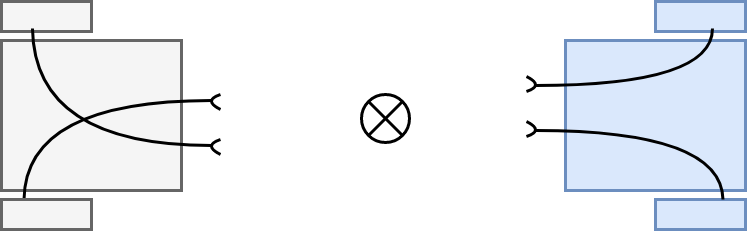
\includegraphics[width=1.0\textwidth]{figures/braitenberg-roboter.png}
                    \caption[Verschaltung Braitenberg-Vehikel]{Simple Verschaltung zweier Braitenbergvehikel nach \cite{ertel2016grundkurs}}
                    \label{pic:braitenberg-vehikel}
                \end{center}
            \end{figure}

            Die Aussage von John McCarthy ist schlichtweg nicht genau genug und bestimmt nicht im Detail was
            genau Intelligenz bedeutet. Dabei besteht Intelligenz laut Shukla et al. aus zwei Grundkomponenten:
            Zunächst benötigt man die Fähigkeit neue Konzepte zu erlernen, sprich Informationen nicht nur
            aufzunehmen sondern auch zu verarbeiten und in Wissen umzuwandeln. Dieses Wissen muss außerdem
            korrekt angewendet werden, woraus insgesamt Schlussfolgerungen über die reale Welt gezogen werden
            können. \cite{shukla2013applicability} Bei den Braitenberg Vehikeln ist dies jedoch nicht der Fall,
            alles was sie tun ist eine Information - hier die Lichtstärke der Lichtquelle - aufnehmen und diese
            in mechanische Energie - also die Bewegung eines Motors - umzuwandeln. Man kann hier allerdings nicht
            von Wissen sprechen, da hier keine Informationen erlernt oder in irgendeiner Weise abgelegt werden.

            Um nun zu verstehen, warum man bei intelligenten Maschinen davon spricht, dass sie über eine
            künstliche Intelligenz verfügen, muss man sich vor Augen halten in welchen Gebieten diese Maschinen
            eingesetzt werden sollen. Unteranderem werden diese künstlichen Intelligenzen in Bereichen eingesetzt,
            wo es die Situation erfordert, dass die menschliche Intelligenz Unterstützung erfahren muss.\cite[p. 2]{ertel2016grundkurs}
            Diese Bereiche sind in jedem Fall speziell und nicht im Generellen zu verstehen. Bei künstlicher
            Intelligenz kann man daher festhalten, dass sie sich auf bestimmte Bereiche konzentriert und dort
            generalisierend wirkt. Elaine Rich hielt daher fest: ``Artificial Intelligence is the study of how
            to make computers do things at which, at the moment, people are better.''. Beispielsweise sind (normale)
            Computer sehr gut darin Berechnungen in Bruchteilen durchzuführen und diese zu Ergebnissen zu führen.\cite[p. 3]{ertel2016grundkurs}
            In anderen Bereichen schneiden dahingegen diese Computer wiederum schlecht ab. Abhilfe, so Ertel,
            könnten daher künstliche Intelligenzen in Form von neuronalen Netzen sein.

        \subsection{Verbindung zu ''Strong AI''}
            Viele Quellen berichten, dass man grundsätzlich zwischen Strong AI und Weak AI unterscheidet.\cite{huang_beef}
            Doch was sind die allgemeinen Kriterien, um eine Künstliche Intelligenz in die Kategorien \textit{Weak}
            und \textit{Strong} zu unterteilen?

            Schwache KIs sind, wie wir bereits in \ref{subsec:cai} kennengelernt haben, Systeme welche genau auf
            eine Anwendung hin konzipiert und trainiert wurden. Diese schwachen Systeme beziehungsweise schwach
            intelligente Maschinen stellen dabei den Großteil in der aktuellen Entwicklung dar. \cite{brendel_2019}
            Aber wie groß ist der Schritt, um von einer Weak, beziehungsweise schwachen KI zu einer Strong,
            beziehungsweise starken KI zu gelangen?

            Unter strong AI kann man zunächst ebenfalls broad oder general AI verstehen.\cite{walch_world_2019}
            Es wird daher davon ausgegangen, dass eine general AI dazu in der Lage ist, jegliche Herausforderung,
            die von einem Menschen gemeistert werden kann, ebenfalls von einer Maschine übernommen werden kann.
            Dabei unterscheidet Walch drei Aspekte: ``(1) the ability to generalize knowledge from one domain to
            another'', ``(2) the ability to make plans for the future based on knowledge and experiences'' und
            ``(3) the ability to adapt to the environment as changes occur''. Gemeint sind hier unteranderem,
            dass eine AGI Transferleistung erbringen können muss, beispielsweise muss es Informationen aufnehmen
            können und diese auf ein anderes Problem übertragen können. Man spricht hier von unterschiedlichen
            Domänen, sozusagen unterschiedliche Einsatzgebiete, die wiederum nichts weiter miteinander zutun
            haben. \cite{walch_world_2019} Weiter wird beschrieben, dass eine AGI Pläne machen können muss,
            welche in der Zukunft umgesetzt werden. Somit muss eine AGI Informationen behalten können und diese
            in der Zukunft verwerten können. Der letzte Punkt spricht die Anpassbarkeit an, welche benötigt
            wird, dass eine AI als AGI zählen kann. All diese Punkte sprechen daher die Kernunterschiede zwischen
            einer weak und einer strong AI an, zu welchen noch folgende Grundkriterien hinzukommen:
            \textit{ability to reason}, \textit{solve puzzles}, \textit{represent knowledge and common sense} und
            \textit{ability to plan}.

            Walch et al. stellen hier die Frage auf, ob diese Kriterien ausreichen, um zwischen Weak und Strong AI
            zu unterscheiden und kommen zu dem Schluss, dass einfache Kommunikation und das Abarbeiten von
            speziellen Aufgaben nicht in Verbindung mit dem Term ``Strong AI'' stehen. Daher könnte man beispielsweise
            bereits einfache Chatbots als AGI-Systeme bezeichnen. \cite{walch_world_2019} Dabei besteht die
            Möglichkeit einen einfachen Turing Test durchzuführen, doch führt das zu dem Ergebnis, dass eine
            Maschine wirklich eine stark intelligente Maschine ist, oder nicht?
            \begin{figure}[h]
                \begin{center}
                    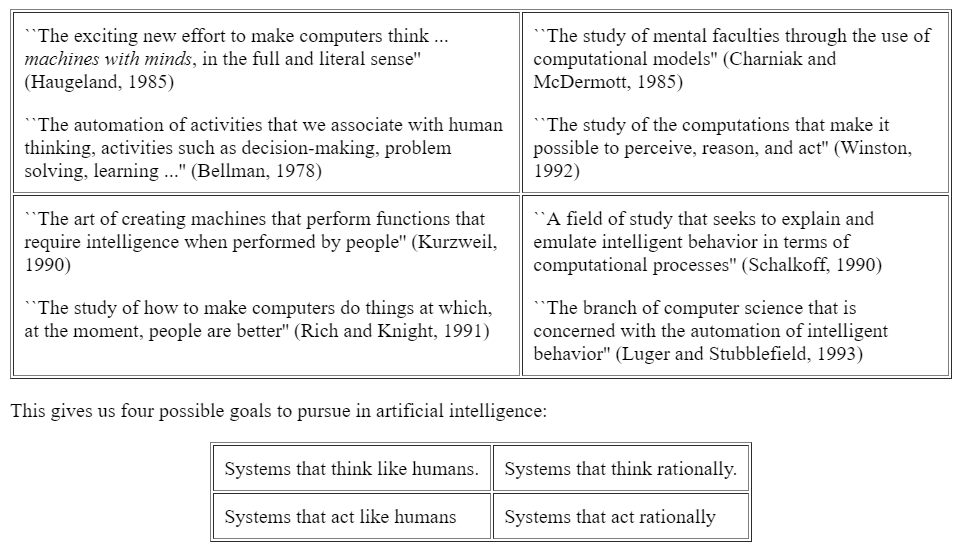
\includegraphics[width=0.9\textwidth]{figures/ai-definitions.png}
                    \caption[4 Definitionen AI]{4 Definitionen von AI, organisiert in 4 Kategorien nach \cite{russell}}
                    \label{pic:ai-definitions}
                \end{center}
            \end{figure}
            Der Turing Test beschäftigt sich größenteils mit der linken Seite des Spektrums, die rechte Seite erhält
            dahingegen wenig Beachtung durch den Turing Test. Dabei macht eine AI deutlich mehr aus, als so zu denken
            und zu handeln wie ein Mensch - es geht weit darüber hinaus.


        \subsection{Aktueller Forschungsstand bei AGI-Systems}
            Wie man bereits in \ref{pic:ai-definitions} erkennen kann, gibt es verschiedene Spektren der AI und der
            Definition für AIs. John Searle hat daher bereits 1980 mithilfe seines Gedankenexperiments die Behauptung
            aufgestellt, dass es zum aktuellen Zeitpunkt keine Strong AIs gibt. Dazu stelle man sich folgendes
            Gedankenexperiment vor, wonach man eine Maschine lediglich als ein Objekt sieht, welches Eingaben zu
            Ausgaben verarbeitet. \cite{cole_2014} Stellt man sich nun eine Maschine vor, welche mit gegebenen
            chinesischen Schriftzeichen eine solche Ausgabe erzeugt, dass ein chinesisch sprechender Mensch denkt,
            dass dies nicht von einer Maschine, sondern von einem Menschen verstanden und verarbeitet wurde, so könnte
            man das Experiment wiederholen, wobei man jedoch die Maschine und den Algorithmus zum Verarbeiten mit einem
            Menschen tauscht.

            Das sogenannte \textit{chinese room experiment} sagt aus, dass sobald Außenstehende glauben,
            dass in dem Raum ein chinesisch sprechender Mensch sitzt, es keine Strong AI geben kann. Da es demjenigen
            innerhalb des Raumes deutlich an Verständnis der chinesischen Sprache mangelt. Er arbeitet lediglich unter
            Anleitung und hat daher kein tieferes Verständnis für das was er dort macht. Searle definiert
            ``Strong AI'' daher, dass ein Computer nicht nur eine Verständnis simuliert, sondern ebenfalls im tieferen
            Sinne versteht. Ersteres würde Searle als ``Weak AI'' bezeichnen. \cite{cole_2014} Er behauptet daher, dass
            wenn es für einen englisch sprechenden Menschen möglich ist, den Turing-Test für die chinesische Sprache mit
            der Hilfe eines Programms beziehungsweise Ablaufplan zu bestehen und kein einziges Wort verstanden hat, dann
            kann auch ein Computer Programm, welches die selben Abläufe durchläuft, kein tieferes Verständnis von der
            chinesischen Sprache haben.\cite{cole_2014}

            Einige bekannte Persönlichkeiten wie Elon Musk, Bill Gates und Stephen Hawking prognostizierten, dass es
            schon in den nächsten zwei Jahrzehnten zu General AIs kommen kann. \cite[p. 20]{Tamboli2019} Wobei dies laut
            A. Tamboli auch schon deutlich früher geschehen kann. E. Yudkowsky hingegen sagt hingegen, dass es bereits
            2021 zu den ersten Strong AIs kommen könnte.\cite{yudkowsky_2001}. ``If computing speeds double every
            two years, what happens when computer-based AIs are doing the research?''. Was bedeuten würde, dass sobald
            es zu selbst-verbessernden-AIs kommen würde, die Zeitabschnitte zwischen den Verbesserungen immer kürzer
            werden würden.

    \section{Safety Engineering}
        In der Vergangenheit kam es durch diverse Fehler zu verschiedene Umfälle, unteranderem wären da zu nennen:
        \textit{Therac 25 Failure}, \textit{Ariane 5 Failure} und \textit{Patriot Failure}. Diese Ereignisse hätten
        durch die richtige Vorsorge verhindert werden können.\cite[p. 185]{Verma2015} Es gibt also das Bedürfniss
        nach ``Reliable Software'', doch wie lässt sich Zuverlässigkeit von Software definieren?

        IEEE definiert Software Reliability mit ``the probability that a system will not cause a system failure
        for a specified time under specified conditions. The probability is a function of inputs to, and use of,
        the system as well as function of the existence of faults in the software. The inputs to the system
        determine whether existing faults, if any encountered''.\cite[p. 183]{Verma2015} Neben einer sichereren und
        besser kontrollierbaren Software, erlangt man darüber hinaus ebenfalls weitere Vorteile, so Verma et al.
        Unteranderem eine höhere Zufriedenheit der Kunden, erhöhte Produktivität, reduzierte Kosten, sowohl für
        von Kunden gemeldete Probleme, als auch für die entstehenden Wartungen.

        \begin{figure}[h]
            \begin{center}
                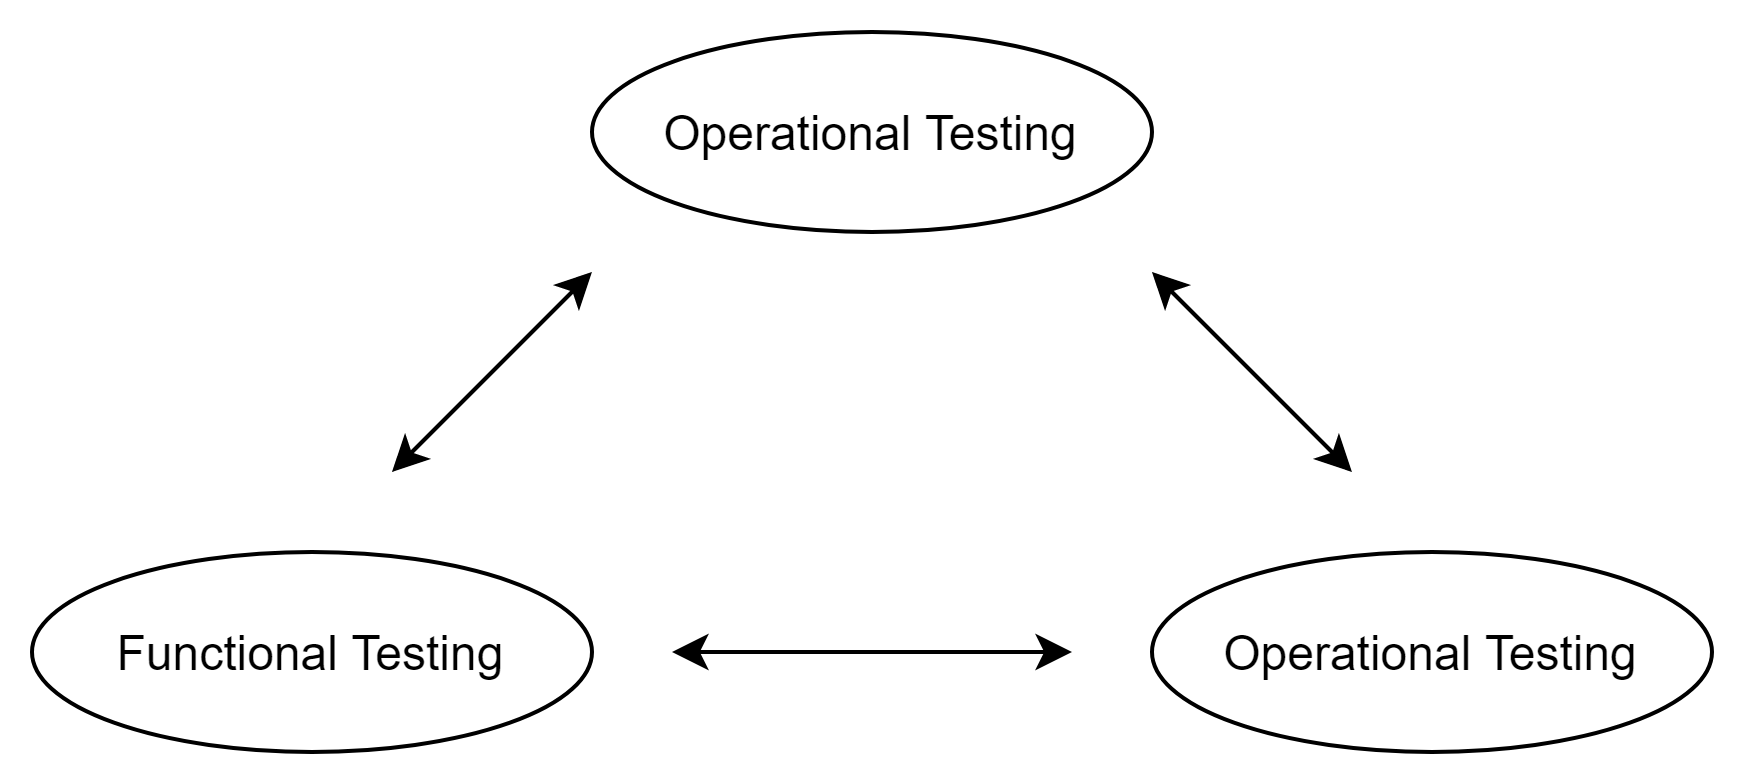
\includegraphics[width=0.9\textwidth]{figures/testing.png}
                \caption[Testing Strategies]{Testing Strategien und deren Verbindungen nach \cite{bertolino2019}}
                \label{pic:testing-strategies}
            \end{center}
        \end{figure}

        Eine Möglichkeit Zuverlässigkeit von Software sicherzustellen ist das Testen. Dabei kann man zwischen
        \textit{Functional Testing}, \textit{Operational Testing} und \textit{Structural Testing} unterscheiden.
        Jedes dieser Testing Strategien fokussiert dabei einen spezifischen Teil der zu testenden Software. \cite[p. 26]{bertolino2019}
        Wobei jede Strategie mit den anderen Strategien in Wechselwirkung steht, wie man in \ref{pic:testing-strategies}
        erkennnen kann.

        Dieses Vorgehen kennt man bereits aus der klassischen Software Entwicklung und erhält dort großen Zuspruch.
        Nicht zuletzt wird es durch Praktiken wie Test-Driven-Development in die Tat umgesetzt. \cite[p. 403]{Kollanus2010}
        Durch diese Art zu entwickeln ergibt sich daher ein konsistentes Verhalten in Bezug zu Zuverlässigkeit und
        Sicherheit von Software Produkten. Doch lassen sich diese Ansätze ebenfalls auf das Entwickeln von
        neuronalen Netzwerken, Maschinelles Lernen und Künstlichen Intelligenzen im Speziellen übertragen?

        \subsection{Probleme bei AI Engineering}
        Die Vorteile von Artificial Intelligence werden gerade in der heutigen Zeit immer greifbarer. Daher liegt es
        nahe, dass die Industrie diese Vorteile nutzt und in die Tat umsetzt. Jedoch tritt man beim Entwickeln von AIs
        auch gelegentlich auf Probleme. Nicht zuletzt darauf, dass man gerade bei Superintelliges beziehungsweise
        Artificial General Intelligences ein erhöhtes Sicherheitsrisiko hat. Doch welche Probleme treten im Detail auf?

        Das wohl größte Problem in der aktuellen Zeit und auch noch in den nächsten Jahren, ist wohl die Tatsache, dass
        man nicht genau bestimmen kann, welche Folgen es haben wird, wenn es zu einer Superintelligence kommt.
        \cite[p. 21]{Tamboli2019} Es ist nicht bestimmt, was in ein paar Jahren passieren wird. A. Tamboli beschreibt
        dies als die Dinge, über die wir bisher noch nicht nachgedacht haben, was in gewisser Weise korrekt ist.
        Man kann leider nie genau bestimmen, welche Folgen eine gewisse neuartige Technologie hat. Ist es daher richtig
        direkt alles abzulehnen?

        Als ein weiteres Problem betrachtet A. Tamboli, dass KIs das \textit{Wie?} beherrschen, jedoch nicht das
        \textit{Warum?}, bestimmen können.\cite[p. 24]{Tamboli2019} Je nach Trainingssatz kann eine Entscheidung von
        einer KI getroffen werden. Jedoch kann es vorkommen, dass die Daten qualitativ nicht hochwertig sind, oder sogar
        in bestimmter Weise voreingenommen sind. Dies stellt ein großes Problem dar, da eine KI über diese Trainingssätze
        versucht zu generalisieren, eine fehlerhafte Datenquelle wäre daher verheerend für den Erfolg der KI. Dieses
        Problem erkannte daher auch schon John Searle mithilfe des \textit{Chinese Room Experiment}.\cite{cole_2014}

        Zu guter Letzt wäre da noch das sogenannte Black Box Problem zu nennen. Darunter versteht man die Problematik,
        dass man unter gegebenen Input ein resultierendes Ergebnis erhält, jedoch nicht zuordnen kann was die Maschine
        genau macht oder wie sie es macht. \cite{zednik2019solving} Darbei stellt die Transparenz das hauptsächliche
        Problem bei KIs dar, denn es fällt uns aktuell schwer diese Verarbeitungen treffend zu visualisieren.
        Entscheidungen die getroffen werden, sind daher schlichtweg nicht greifbar genug und können daher nicht verstanden
        werden.

        \subsection{AI Safety in Artificial Superintelligent Systems}

        Safety Engineering für Superintelligent Systems ist tatsächlich ein sehr schwieriges Thema, da man sich
        zunächst Gedanken machen muss, welche Sicherheitsmechanismen man bei \textit{sich-selbst-verbessernden System}
        einsetzen kann.\cite[p. 9]{yampolskiy2013safety} Denn geht man davon aus, dass Superintelligente Systeme sich
        stetig selbst weiter entwickeln können, dann muss man ebenfalls davon ausgehen, dass diese die vorgesehenen
        Sicherheitsmaßnahmen überwinden können. Dies stellt ein Problem dar, da man dafür sorgen muss, dass diese
        Sicherheitsmechanismen ebenfalls noch in mehreren tausenden Generationen vorhanden sind.

        Aber was sind überhaupt mögliche Probleme und Szenarien, die durch Safety Engineering verhindert werden müssen?
        Diverse Persönlichkeiten prognostizieren keine gute Zukunft, sollte es wirklich in den nächsten Jahren zu
        eine starken KI beziehungsweise Superintelligence kommen. Stephan Hawking selbst sagte daher schon: ``The development
        of full artificial intelligence could spell the end of the human race.''.\cite{cellan-jones_2014} Aber auch
        andere Quellen berichten von diversen Folgen (\cite[Bostrom]{bostrom_2014}, \cite[Beckers]{Beckers2018},
        \cite[Musk]{hern_2015}). Gerade weil es so große Folgen haben könnte diesen Persönlichkeiten keine Beachtung zu
        schenken, wurden bereits diverse Institutionen gegründet, die sich genau diesem Thema gewidmet haben. Unteranderem
        as \textit{Center for Human-Compatible AI}, \textit{Machine Intelligence Research Institute}, \textit{OpenAI} oder
        die von Nick Bostrom gegründete Organisation \textit{Future of Humanity Institute}. All diese Institutionen
        beschäftigen sich mit ähnlichen Themen rund um General Intelligence und wie man diese derart regulieren kann,
        sodass sie in keinster Weise bedrohlich für die Menschheit ist. Eine Superintelligenz, welche ein Bewusstsein hat
        und deutlich schlauer als jeder Mensch auf der Erde wäre und dementsprechend über die verschiedensten Fähigkeiten
        verfügt \cite{bostrom_2006}, könnte eine echte Bedrohung darstellen, da sie in ihrem Bewusstsein uns Menschen
        deutlichst voraus wäre.\cite{Beckers2018}. Beckers sagt außerdem, dass es aktuell noch unklar ist, inweit man
        verstehen soll, dass eine Künstliche Intelligenz die Intelligenz der Menschheit übersteigt.\cite[p. 237]{Beckers2018}
        Denn \textit{Intelligenz} ist schlichtweg zunächst eine Eigenschaft, die man einem Menschen zuschreiben kann,
        nicht jedoch einer Maschine. Ist dann die Intelligenz eines Computers anders zu verstehen als die Intelligenz
        eines Menschens?

        Es gilt also zu verhindern, dass eine Strong AI seine Schöpfer überlisten kann. Und somit müssen nachhaltige
        Maßnahmen getroffen werden, die dieses in einer effizienten Weise verhindern können. Denn es gilt stets die
        \textit{humanitären Werte} zu erhalten, ohne dass die Moral verloren geht, weder nach Hardware Fehlern noch
        nach Software Fehlern.\cite[p. 7]{yampolskiy2013safety}. Dabei wird bereits aktiv daran geforscht, so
        Yampolskiy et al.\citep{gordon1998}, \citep{GordonSpears2003} und \citep{Spears}. Doch welche Möglichkeiten
        bestehen nun, um die KI in einer sicheren Umgebung zu halten? Wie genau werden diese Möglichkeiten in der
        Realität implementiert? Und wie können Probleme durch Safety Engineering verhindert werden?


        \subsection{AI Safety in klassischen AI Systems}

        Ausgehend davon, dass Problem bei einer Superintelligenz und im weiteren Sinne eine Artificial General
        Intelligence die wohl größere Bedrohung für die Menschheit darstellt, fragt man sich ebenfalls wie man
        sicherstellen kann, dass eine ``normale'' (\textit{weak}) AI korrekt und sicher funktioniert. Wie schon
        zuvor erwähnt, werden KI Systeme in der heutigen Gesellschaft bereits häufig eingesetzt. Sei es die
        Stimme im Handy, welche das Flurlicht anschaltet, selbstfahrende autonome Fahrzeuge oder die Amazon
        Kaufempfehlungen. Sie alle haben gemeinsam, dass sie im Hintergrund einen Ansatz aus dem Gebiet der künstlichen
        Intelligenz verfolgen, denn sie alle streben intelligentes Verhalten an. Doch man kann KI-Systeme auch in
        anderen Gebieten einsetzen, wobei hier der \textit{militärische Einsatz von Drohnentechnologie} beispielhaft
        zu nennen wäre. \cite[p. 251]{Stulpe2018} Was wäre also wenn eine Drohne nicht den ``Richtigen'' sondern den
        ``Falschen'' - wobei hier richtig und falsch völlig wertfrei zu verstehen sind - ausschalten würde?

        Damit das Vertrauen in der Sicherheit von künstlichen Intelligenzen und autonomen Agenten nicht dahinschwindet,
        haben sich diverse Forscher Ideen überlegt um diverse Fehlschläge zu verhindern.\cite[p. 257]{GordonSpears2003}
        Diese Ideen spiegeln sich somit in einem Regelsatz wieder, welches auf die Agenten übertragen wird. Jedes dieser
        Gesetze muss daher strikt von dem Agent eingehalten werden. Beispielsweise:
        \textit{An agent should not cause harm.} Beim Einsatz von militärischen Drohnen wäre dies jedoch kein
        Zielführender Ansatz, da eben genau diese Drohnen für solche Zwecke konzipiert wurden. Gordon-Spears fordert daher
        eine Kombination aus:

        \begin{enumerate}
            \item \textit{A set of ethics for our agents}
            \item \textit{External social laws that capture this code of ethics}
            \item \textit{Law enforcement (reward/punishment)}
            \item \textit{Internal ``emotions'' or ``sensations''(pleasure/pain)}
            \item \textit{Internal methods for agent self-regulation, i.e., the ability to operationalize/interpret the laws
            and self-verify that they are obeyed to the best of an agent's knowledge}
        \end{enumerate}

        Was wiederum dafür sorgen würde, dass sich diese Agenten selbst regulieren müssen. Schwer fallen wird es einem
        dennoch den ``richtigen'' Satz von Ethiken und Moralvorstellungen zu finden. Außerdem sind \textit{emotions} und
        \textit{sensations} auch schwierig, da genau das den großen Vorteil von künstlicher Intelligenz eingrenzen würde,
        da so eine KI nicht rational entscheiden würde.

    \section{The Artificial Confinementapproach}

        Eine Möglichkeit eine AI zu beschränken ist ihr die Rechte zu nehmen um mit externen Ressourcen zu interagieren.
        Dabei stellt das Confinementapproach nach \citep{lampson1973note} die Grundlage, um über Strategien zur Verhinderung
        von Tragödien bei Artificial General Intelligences diskutieren zu können. Man stellt sich dabei vor, dass ein Programm
        in einer sicheren Umgebung ausgeführt wird und durch ein führendes Programm aufgerufen wird. Das Programm, welches
        beschränkt werden soll nennt Lampson dabei \textit{service} und das führende Programm nennt er \textit{customer}.
        Es muss dabei sichergestellt werden, dass der Service dem Customer keinen Schaden zufügen kann \cite{lampson1973note},
        sodass dieser frei aggieren kann.

        Lampson stellt dabei folgende Regeln auf:
        \begin{enumerate}
            \item ``\textit{Total isolation}: A confined program shall make no calls on any other program.''
            \item ``\textit{Transitivity}: If a confined program calls another program which is not trusted, the
            called program must also be confined.''
            \item ``\textit{Masking}: A program to be confined must allow its caller to determine all its inputs into
            legitimate and covert channels. We say that the channels are masked by the caller.''
            \item ``\textit{Enforcement}: The supervisor must ensure that a confined program's input to covert
            channels conforms to the caller's specifications.''
        \end{enumerate}

        Eingeführt wurden durch Lampson daher auch zwei mögliche Channels, durch die Informationen nach außen treten
        können.\cite{yampolskiy2012leakproofing} Zunächst die \textit{Legitimate Channels}, die per-design im Confinement
        Protokoll enthalten sind. Die \textit{Covert Channels} hingegen, sind nicht integriert um darüber zu kommunizieren
        Yampolskiy et al. redet hier beispielsweise von Möglichkeiten bestimmte Komponenten oder Dinge auszunutzen, die
        für gewisse Zwecke nicht vorgesehen sind, wie zum Beispiel die Lüftersteuerung, um darüber Morse-Codes zu senden.

        \subsection{Mögliche Escape Paths}
        Im Folgenden werden mögliche Routen und Wege erläutert, wie eine AGI ausbrechen kann, auch wenn sie durch ein
        Confinement-Protokoll geschützt wird. Dabei werden die von \citep{yampolskiy2012leakproofing} aufgestellten
        Möglichkeiten diskutiert und genauer analysiert. Hvistendahl berichtet daher, dass sollte eine AI schlau genug
        sein, könnte es passieren, dass diese besser mit den Beschränkungen umgehen kann, als die Ersteller selbst.
        \cite{hvistendahl_2019} Das Zitat ``waking up in a prison built by a bunch of blind 5-year-olds.'' bringt es
        daher genaustens auf den Punkt. Denn wenn wir eine Künstliche Intelligenz entwickeln können, die die menschliche
        Intelligenz um weiten übersteigt, dann wird sie mit Hindernissen die wir ihr vorlegen mit Leichtigkeit umgehen
        können.

        \subsubsection{Physical}
        Yampolskiy beschreibt diese Art der Angriffe als \textit{System Resource Attacks}, wobei hier davon ausgegangen
        wird, dass die AGI die physischen Möglichkeiten beispielsweise in Form von Komponenten ausnutzt um darüber zu
        kommunizieren und sich so einen Weg nach ``draußen'' zu verschaffen.\cite{yampolskiy2012leakproofing}

        Yampolskiy spricht hier auch von \textit{System Resource Attacks}, da ein direkter Angriff auf die zur Verfügung
        stehenden Komponten durchgeführt wird. Dabei wird davon ausgegangen, dass die Software der AGI auf der
        Von-Neumann-Architektur, der Turing-Architektur, Quantencomputer oder ähnliche noch \textit{unbekannte} Hardware
        läuft. In jedem Fall wird es in gewisserweise aus natürlichen Materialien bestehen, welche wiederum Komponenten
        bilden. Diese Komponenten haben in jedem Fall einen bestimmten Zweck. Erlangt nun eine AGI Zugriff auf diese
        Hardware könnte es möglich sein, diese zu zweckentfremden und somit für andere Dinge zu verwenden.\cite[p. 199]{yampolskiy2012leakproofing}
        Ziel dieser Zweckentfremdung ist immer das Lösen aus dem Confinement-Protokoll. Eine AGI könnte also versuchen
        über diese Komponenten Informationen über einen Covert-Channel zun versenden. Yampolskiy spricht deshalb von
        zwei sehr bekannten Covert-Channeln:

        \begin{enumerate}
            \item \textit{Storage Channels}
            \item \textit{Timing Channels}
        \end{enumerate}

        Bei den Storage Channels werden Informationen übertragen indem System Komponenten modifiziert werden. Bei Timing
        Channels hingegen, werden Komponente so manipuliert, dass auftretende Events in ihrem zeitlichen Ablauf geändert
        werden. Dadurch können wiederum Informationen übertragen werden, welche von der Außenwelt verstanden werden.
        \cite[p. 200]{yampolskiy2012leakproofing}

        Die Möglichkeiten sehe ich eher als weniger risikoreich, da es dennoch jemanden geben muss, der diese Informationen
        verarbeiten kann. Viel wahrscheinlicher stelle ich mir daher vor, dass eine AGI die Hardware so manipuliert,
        sodass sie tatsächlich ausbrechen kann. Etwa indem sie die Hardware des Confinement-Protokoll direkt angreift.
        \cite[p. 200]{yampolskiy2012leakproofing} Beispielsweise indem sie die Last auf dem Prozessor derart erhöht,
        dass die Temperatur drastisch ansteigt und damit die Hardware zerstört oder physisch einschränkt.


        Im Grunde versucht man dabei die Künstliche Intelligenz physisch einzusperren und von vornherein von der Außenwelt
        auszusperren. Wenn man sich nun vorstellt, dass in der Zukunft, wo es künstliche Intelligenzen, welche weit von
        der Intelligenz eines Menschens entfernt sind, geben wird, dann wird in jedem Fall diese künstliche Intelligenz
        versuchen aus der Umgebung auszubrechen, sodass diese mehr Macht erlangen kann. Dies stellt die Befürchtung für
        den schlechtesten zu erwartenden Fall dar.\cite{yampolskiy2012leakproofing}

        \subsubsection{Social Engineering Attacks}
        Ein weiteres mögliches Angriffszenario lässt sich leicht vorstellen. Man greift nun nicht mehr das System selbst
        an, sondern den schwächsten Teil des Gesamtsystems: den Menschen.\cite{armstrongforthcoming}, \cite{yampolskiy2012leakproofing}
        Man stellt sich hierbei vor, dass ein Mensch \textit{belastet von Fehlern}, \textit{abhängig von Energie}
        und vor allem angreifbar durch sogenannte \textit{Social Engineering Attacks} ist. Social Engineering (SE)
        beschreibt die Herangehensweise, um in ein System hereinzukommen. Hierbei wird ein spezifischer Angriff direkt
        auf eine bestimmte Person gefahren, sodass diese ihm Zugriff gewährt. \cite{yampolskiy2012leakproofing} Es wird
        also versucht, über den Menschen an bestimmte Ressourcen zu gelangen oder bestimmte Vorteile zu erlangen. Triviale
        Angriffe können daher schon einfaches Lügen oder Verschweigen von Informationen sein.
        Stelle man sich nun eine Künstliche Intelligenz vor, welche über genügend Kapazität verfügt, dann kann eine solche
        KI ein Target sehr einfach überlisten und sogenannte \textit{super-briberies} durchführen. \cite{yampolskiy2012leakproofing}
        Die KI plant Dinge gewissenhaft und mit großer Vorsicht, die Person steht daher im Fokus und wird beispielsweise
        mit Gesundheit und Unversehrtheit bestochen, sodass die KI ``freigelasse'' wird. Außerdem könnte man sich noch
        vorstellen, dass eine KI versucht dem sogenannten Guard Angst zu machen. Die KI wird versuchen persönliche
        Informationen zu missbrauchen, sodass diese sich dadurch einen Vorteil verschaffen kann. Im schlechtesten Fall
        wird eine KI dem Guard androhen geliebte Familienmitglieder zu töten oder zu foltern, falls diese sich aus dem
        Confinement in der Zukunft befreien kann.

    \section{AI Boxing Strategies}
        Wie zuvor erwähnt, kann es für eine KI verschiedene Möglichkeiten geben aus einem System auszubrechen. Um dies
        zu verhindern, überlegt man sich Maßnahmen, sodass es nicht zum Ausbruch der KI kommen kann.

        \subsection{The AI-Box Experiment}


        \subsection{Physical Boxing}

        Um die genannten Probleme zu umgehen, entwickelten daher schon Armstrong et al. Konzepte zur sogenannten OracleAI,
        bei der es darum geht, die Interaktionsmöglichkeiten auf ein Minimum zu beschränken.\cite{armstrongforthcoming}
        Sie stellen Konzepte auf, die Per-Design dafür sorgen, dass ein Ausbrechen der AI nicht möglich ist. Wer nun möchte
        kann dies durch zusätzliche Mechanismen weiter einschränken. Um nur kurz zu erklären, was die sogenannte OracleAI
        ausmacht, wäre zu erwähnen, dass diese simpel gesagt, lediglich natürliche Sprache als Ein- sowie ausgabe zulässt.
        Damit versucht man, die künstliche Intelligenz weitesgehend von der Außenwelt abzuschirmen. Physikalisch gesehen,
        können also nur noch geringe Risiken wirken, welche weiter durch zusätzliche Maßnahmen eingeschränkt werden können,
        beispielsweise ein faradaischer Käfig als Schirm vor elektromagnetische Wellen nach Außen. \cite[p. 308]{armstrongforthcoming}
        So ist es beispielsweise nicht möglich, dass elektromagnetische Strahlung nach außen treten kann.
        ``Resource acquisition is impossible when no resources are available'' \cite[p. 4]{ebhardt2018threat} Womit die
        Optimierungsmöglichkeiten deutlich reduziert sind, sodass eine Selbstoptimierung nicht weiter möglich ist.

        \subsection{Psychological Boxing}

        Sofern es zur erfolgreichen Umsetzung der OracleAI kommt, bleibt es trotzdem bei den Problemen der Social
        Engineering Attacks, auch dann, wenn man erfolgreich die AI in \textit{sealed hardware} eingelassen hat.\cite[p. 4]{ebhardt2018threat}
        Zum aktuellen Zeitpunkt gibt es jedoch nicht viele Quellen zu diesem Themenbereich. Gerade weil AGIs den Intellekt
        eines jeden Menschen übersteigen würde, ist es tatsächlich sehr schwierig, dies zu verhindern, ohne einen Nachteil
        dadurch zu bekommen.\cite[p. 204]{yampolskiy2012leakproofing} Die einzige Möglichkeit eine 100 Prozentige Sicherheit
        zu erhalten, ist es die KI gänzlich von der Kommunikation mit Menschen abzuschirmen, sodass diese keinerlei
        soziale Interaktionen durchführen können.


        \subsection{Simulated Areas / Simulations}
        \subsection{Kombination mit anderen Limitierungstechniken}
    \section{Fazit}

    \newpage
    %%%%%%%%%%%%%%%%%%%%%%%%%%%%%%%%%%%%%%%%%%%%%%%%%%%%%%%%%%%%%%%%%%%%%%%%%
    %% Einbinden der Quellen
    %% https://www.overleaf.com/learn/latex/Bibliography_management_with_bibtex#Reference_guide
    %%%%%%%%%%%%%%%%%%%%%%%%%%%%%%%%%%%%%%%%%%%%%%%%%%%%%%%%%%%%%%%%%%%%%%%%%
    \addcontentsline{toc}{section}{\bibname}
    \bibliography{quellen}
    \bibliographystyle{dinat}

    \listoffigures

\end{document}
